\chapter{Typsystem}
\label{ch:Typsystem}
Der Datentyp einer Variable oder Konstante beschreibt den Inhalt der Daten und teilt dem Compiler mit, wie diese Daten behandelt werden können. 
Anhand des Datentyps weiß der Compiler wieviel Arbeitsspeicher er reservieren muss und kann sicherstellen das einer Variable keine falschen Daten zugewiesen werden \cite[S.62]{Mathias.2016}.

\section{Basidatentypen}
Sowohl Go als auch Swift bringen die grundlegenden Datentypen mit, die auch von anderen Hochsprachen gewohnt sind.
In \autoref{tab:DatentypenGo} sind die in Go verfügbaren Datentypen aufgelistet.

\begin{table}[H]
    \centering
    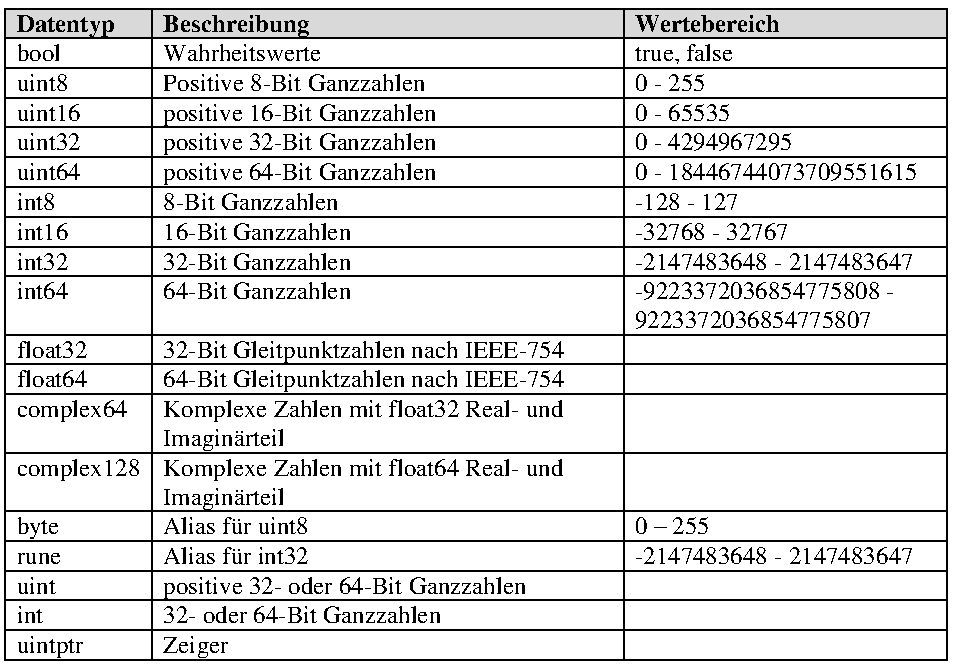
\includegraphics[width=\textwidth]{Tabellen/Datentypen_Go.pdf}
    \caption{Datentypen in Go}
    \label{tab:DatentypenGo}
\end{table}

Die Ganzzahl-Datentypen können jeweils als 8-, 16-, 32- oder 64-Bit-Variante verwendet werden. 
Wird kein spezieller ganzzahliger Datentyp definiert, sondern nur ein \emph{int} oder \emph{uint} so kommt es darauf an, ob das Programm auf einem 32-Bit oder 64-Bit System kompiliert wird.
Wird auf einem 32-Bit-System eine Variable als \emph{int} deklariert ist diese jedoch nicht automatisch auch vom Typ \emph{int32}.
Im \autoref{lst:VariablenGo} ist dies beispielhaft dargestellt. 
Beim kompilieren von \autoref{lst:VariablenGo} gibt der Compiler die in Zeile 9 dargestellte Fehlermeldung aus. 
Die beiden Typen \emph{byte} und \emph{rune} sind Alias-Datentypen.
Der Typ \emph{rune} wird üblicherweise für Unicode-Zeichen benutzt, um sich semantisch von dem numerischen Datentyp \emph{int32} zu unterscheiden. 
Gleichermaßen verhält es sich mit dem Typ \emph{byte}, der dafür benutzt werden sollte Rohdaten abzulegen anstatt eines numerischen Wertes \cite[S.98]{Kennedy.2016}.

\begin{listing}[H]
\caption{Implizite und explizte Angabe des Datentypen in Go}
\label{lst:VariablenGo}
\begin{GoCode}
package main

func main() {
    var x int = 3
    var y int32 = 4

    var result = x + y	
}
//invalid operation: x + y (mismatched types int and int32)
\end{GoCode}
\end{listing}

Ebenso wie Go bietet Swift dem Programmierer an ein 

\begin{listing}[H]
\caption{}
\end{listing}

\begin{table}[H]
    \centering
    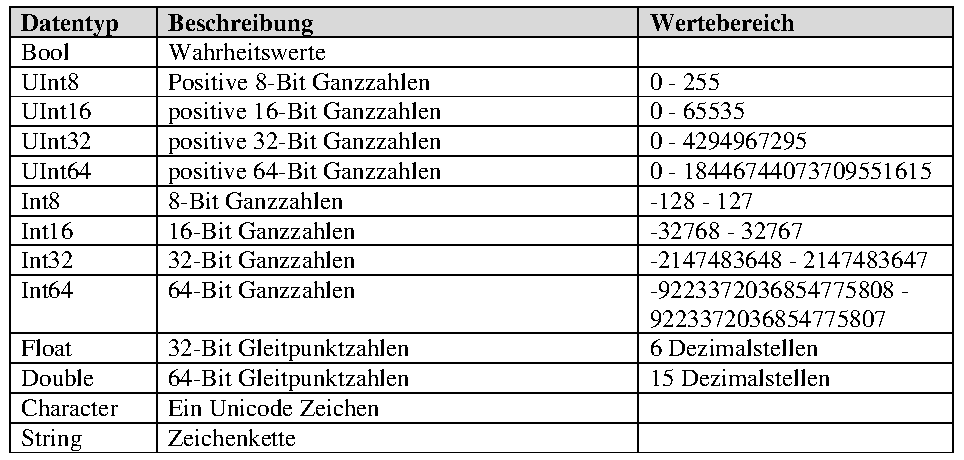
\includegraphics[width=\textwidth]{Tabellen/Datentypen_Swift.pdf}
    \caption{Datentypen in Swift}
    \label{tab:DatentypenSwift}
\end{table}

\section{Type Inference}
\label{sec:TypeInference}
Beide Sprachen beherrschen Type Inference. 
Durch Type Inference ist es nicht nötig den Datentyp einer Variable anzugeben, sondern der Compiler erkennt diesen anhand des zugewiesenen Wertes. \cite[S.307]{Hinzberg.2015}

\section{Zeichenketten}

\section{Arrays}

\section{Erweiterte Datenstrukturen}


